% main.tex
% !TeX program = lualatex
% !BIB program = biber

\documentclass[12pt,letterpaper]{report}

\usepackage[spanish,es-nodecimaldot]{babel}
\usepackage{csquotes}
%referencias bib
\usepackage[
  backend=biber,
  style=verbose-trad2,    % notas al pie completas + 'Ibíd.' / 'Op. cit.'
  autocite=footnote,      % \autocite => nota al pie
  ibidtracker=context,    % controla cuándo usar Ibíd.
  pagetracker=true
]{biblatex}
\addbibresource{referencias.bib}

\AtEveryCite{%
  \togglefalse{bbx:url}%
  \togglefalse{bbx:doi}%
  \togglefalse{bbx:eprint}%
  \togglefalse{bbx:isbn}%
  \renewbibmacro*{url+urldate}{}% suprime tanto la URL como la fecha de consulta en la nota
}

\usepackage{icontec_style}
\usepackage[hidelinks]{hyperref}

%Ajustes de cleveref
\usepackage[spanish,noabbrev,nameinlink]{cleveref}

%Configuraciones extra para referencias al español
\DefineBibliographyStrings{spanish}{references = {Referencias},}
\DefineBibliographyStrings{spanish}{
  ibidem = {Ibíd.},
  opcit  = {Op.\addabbrvspace cit.},
}

\usepackage[hang,flushmargin]{footmisc}
% --- Espaciado de notas al pie ---
\setlength{\footnotesep}{14pt}              % separación ENTRE notas
\setlength{\skip\footins}{14pt plus 4pt}    % separación del texto al bloque de notas
\renewcommand{\footnotelayout}{\setstretch{1}}

% Metadatos portada:
\icontecsetup{
  universidad = {Universidad Industrial de Santander},
  facultad    = {Facultad de Ingenierías Fisicomecánicas},
  programa    = {Escuela de Ingeniería de Sistemas e Informática},
  titulo      = {PROTOTIPO DE UN VIDEOJUEGO SERIO SOBRE SISTEMAS FERROVIARIOS EN COLOMBIA},
  autores     = {\\Miguel Ángel Plata Rodríguez -- 2190050\\Mateo Salazar Serrano -- 2200135},
  director    = {\\Urbano Eliécer Gómez Prada, PhD},
  ciudad      = {Bucaramanga},
  anio        = {\textit{(poner fecha de entrega)}}
}

\begin{document}

% Portada
\maketitleicontec

%Agradecimientos / Resumen / Abstract
% \chapter*{Agradecimientos}\addcontentsline{toc}{chapter}{Agradecimientos}
% \begin{resumen} ... \keywords{...} \end{resumen}
% \begin{abstractES} ... \keywords{...} \end{abstractES}

% Índices
\tableofcontents
\listoffigures
\listoftables
\clearpage

% ===== Contenido =====
% !TeX root = ../main.tex

\chapter{Introducción}

\section{Introducción}
El transporte ferroviario a lo largo de la historia ha desempeñado un papel fundamental para el desarrollo económico y logístico de los países industrializados. Colombia, a pesar de haber sido pionera en la introducción del ferrocarril en América Latina, ha presentado un estancamiento significativo a lo largo de las ultimas décadas, producto de la priorización de la infraestructura vial y de debilidades institucionales y técnicas en el sector. Según datos del ministerio de transporte, mas del 60\% de la red ferroviaria nacional se encuentra inactiva, y el modo férreo apenas representa el 0.1\% de la carga nacional movilizada.

En los últimos años, han resurgido iniciativas como el corredor de La Dorada-Chiriguaná, el Regiotram de Bogotá y el Tren de Cercanías del Valle del Cauca, que evidencian un renovado interés por revitalizar el sistema férreo colombiano. En este contexto, la aplicación de tecnologías interactivas, como los videojuegos educativos, emerge como una alternativa viable para fomentar la comprensión y el interés de las personas sobre los desafíos técnicos, económicos y sociales asociados al desarrollo ferroviario.

En este contexto, el Game Based Learning (GBL) surge como una iniciativa pedagógica prometedora, proponiendo el uso de entornos interactivos y dinámicos para promover la adquisición de conocimientos mediante la experiencia y la retroalimentación. Por su parte, los videojuegos serios se desarrollan con fines más allá del entretenimiento, integrando objetivos pedagógicos y simulaciones realistas. Estas herramientas permiten representar de forma didáctica problemas complejos del mundo real, como los que enfrenta la infraestructura férrea del país.

Este trabajo de grado tiene como objetivo el desarrollo de un prototipo de videojuego serio orientado a la comprensión de los desafíos asociados al desarrollo ferroviario en Colombia. Implementado mediante el motor grafico Unity 6 y el software de modelado Blender se busca crear una experiencia educativa que incorpore los criterios esenciales del GBL: inmersión, interacción, control del aprendiz, apoyo del aprendizaje, narrativa y evaluación.


\section{Planteamiento y justificación del problema}
Colombia, a pesar de haber sido pionera en la introducción del ferrocarril en Latinoamérica, se ha visto estancada en su desarrollo ferroviario. Tras una búsqueda en la plataforma web de la Agencia Nacional de Infraestructuras sobre los proyectos activos \autocite{aniProyectos}, de los 133 proyectos activos, sólo 4 son proyectos ferroviarios, de los cuales 2 llevan desde 1998 y 1999 en operación. Además, según datos del Ministerio de transporte de Colombia \autocite{mintransporteSurcos2024}, el 63,2\% de la red ferroviaria nacional se encuentra inactiva y, excluyendo el transporte de carbón y petróleo, el modo ferroviario apenas representa el 0,1\% de la carga nacional movilizada, lo cual evidencia una falta de interés e iniciativa por parte de los gobiernos que, a su vez, ha derivado en una priorización de la inversión pública en la infraestructura de carreteras \autocite{mintransporteDatosCarga}.

Según la monografía \textit{Desafíos del transporte ferroviario de carga en Colombia}, la dificultad en desarrollar efectivamente un transporte ferroviario en Colombia es debido a factores como los conflictos políticos, el manejo de los recursos y de la debilidad ingenieril del sector. Específicamente se menciona: “La institucionalidad del sector presenta hoy debilidades en materia de planeación y política ferroviaria; ingeniería ferroviaria conceptual…” \autocite[p.~17]{iabdDesafios}.

Actualmente, hay que considerar que recientemente la nación está intentando reiniciar el desarrollo de infraestructuras ferroviarias. Algunos de los proyectos que evidencian este reciente interés son: la firma del contrato de concesión, la primera Asociación Público-Privada (APP) del país, correspondiente al corredor de La Dorada–Chiriguaná \autocite{mintransporteAPP2025}; el inicio de las obras del Regiotram de Occidente, que beneficiará a Bogotá y a sus municipios aledaños \autocite{bogotaRegiotram2025}; y el megaproyecto del Tren de Cercanías del Valle del Cauca \autocite{valoraTrenValle2024}, que busca conectar Cali con Jamundí, Yumbo y Palmira.

Aun así, ante la carencia de herramientas que refuercen la planeación y la ingeniería ferroviaria, resulta oportuno desarrollar recursos que impulsen el aprendizaje y la concientización sobre los desafíos de este sector.

Los videojuegos en su mayoría se enfocan en el entretenimiento del jugador, sin embargo, existe la posibilidad de diseñar juegos educativos, tal es el caso de un estudio descrito en el artículo “Examining the characteristics of game-based learning: A content analysis and design framework” \autocite{gblFrameworkExamining} en donde, a partir del análisis y la codificación de 194 artículos diferentes sobre juegos educativos, se definió un marco de diseño de un \textit{Game-Based Learning} (GBL), o aprendizaje basado en un juego.

Un GBL se compone por dos grupos de características, las primarias y secundarias, siendo las primarias los aspectos que se consideran esenciales para un juego educativo \autocite{gblFrameworkExamining}: Criterios de inmersión, interacción, control del aprendiz, apoyo al aprendizaje, narrativa y evaluación.

Además, según el libro \textit{Serious Games: Mechanisms and Effects}, se define un videojuego serio como “cualquier forma de software de juego interactivo basado en computadora (…) y que se ha desarrollado con la intención de ser más que entretenimiento.” \autocite[p.~6]{seriousGamesMechanisms}. Aspecto que aplica para el caso de estudio de este proyecto, ya que se tiene planteado, además de entretener, educar sobre los desafíos del desarrollo ferroviario en Colombia.

Al respecto, existen diversos antecedentes de videojuegos de simulación enfocados en diseñar y construir sistemas férreos, como son el \textit{Railway Empire} \autocite{railwayEmpire} ambientado en Estados Unidos entre siglo XIX y XX, \textit{Railroad Tycoon 3} \autocite{railroadTycoon3} basado en escenarios para recrear sistemas férreos importantes en la historia de la humanidad y \textit{Train Valley 2} \autocite{trainValley2} enfocado en la resolución de puzles; sin embargo, ninguno de los videojuegos mencionados tiene propósitos más allá del entretenimiento, objetivo que sí se busca en este proyecto de grado.

Tras una búsqueda con el motor Google Academics y usando la ecuación: (“Colombia” AND “Sistema Férreo” AND (“Videojuego Serio” OR “Videojuego de simulación” OR “Videojuego educativo”)), se encontró solamente una tesis de grado que tenía como objetivo “Investigar sobre interfaces hápticas para aplicaciones 3D, así como analizar su interactividad y usabilidad en una aplicación interactiva para la maqueta de transportes ESPOCH.” \autocite{tesisInterfacesHapticas}, en el que no es un aspecto suficiente para que sea considerado el desarrollo de un videojuego serio, ya que en ningún momento describe el proceso de desarrollo de un videojuego, solo se menciona como un ejemplo. En ese orden de ideas, se puede concluir que no se encontró ningún videojuego serio de sistemas ferroviarios ambientado en Colombia.

Por lo anterior, se formula la siguiente pregunta de investigación:

\textbf{¿Cuál debería ser la estructura de un prototipo de videojuego serio sobre los desafíos del desarrollo del sistema ferroviario en Colombia y cómo se implementaría para que tenga en cuenta los criterios de inmersión, interacción, control del aprendiz, apoyo al aprendizaje, narrativa y evaluación del marco GBL?}

En el orden de ideas de lo manifestado, se puede considerar viable una iniciativa en el desarrollo de un prototipo de software para la educación del sector ferroviario, por lo tanto, se propone implementar un primer prototipo de un videojuego serio de sistemas ferroviarios en Colombia, con el fin de concientizar la comprensión de algunos de los desafíos que conllevaría la planeación y el desarrollo de la infraestructura férrea en el país.

Se espera que el prototipo del videojuego serio sobre los desafíos del sistema ferroviario en Colombia incorpore las características primarias del marco GBL como la evaluación (cómo se mide el aprendizaje), la inmersión (cuán envolvente es el entorno del juego), la interacción (cómo se comunica el jugador con el juego o entre jugadores), el control del aprendiz (el grado de autonomía que tiene el usuario), el apoyo al aprendizaje (tutoriales y ayudas) y la narrativa (la historia o contexto que da sentido a la experiencia). Estas características se usarán para “ayudar a trazar rutas de aprendizaje más personalizadas, motivadoras y potencialmente efectivas para el aprendizaje.” \autocite[p.~10]{gblHandbook2019}.

El prototipo tendrá una prueba piloto dirigida a estudiantes UIS, con el objetivo de evaluar la experiencia del jugador y el desempeño del software. La prueba se orientará a determinar si el prototipo resulta agradable en su uso y se encuentre libre de errores, permitiendo identificar áreas de mejora para quienes deseen dar continuidad a este proyecto.

\section{Objetivos}

\subsection{Objetivo General}
Desarrollar un prototipo de un videojuego serio para la comprensión de algunos de los desafíos que conllevaría el mejoramiento de la infraestructura férrea en Colombia, usando GBL, Unity 6, Blender y RUP adaptada con elementos de Kanban.

\subsection{Objetivos Específicos}
\begin{enumerate}[label=\arabic*.]
  \item Definir las historias de usuario del videojuego serio a partir del marco GBL para el apoyo de la comprensión de algunos de los desafíos del desarrollo férreo.
  \item Diseñar los componentes que integran el videojuego serio tales como los sistemas de evaluación, inmersión, interacción y control del jugador a partir del contexto de sistemas ferroviarios en Colombia.
  \item Implementar el videojuego serio integrando un sistema interactivo de un mapa 3D, así como eventos ambientales, económicos y sociales usando Unity 6 y Blender.
  \item Evaluar el videojuego serio realizando pruebas de funcionalidad y usabilidad.
\end{enumerate}

% !TeX root = ../main.tex

\chapter{Marco de referencia}

\section{Sistemas Ferroviarios en Colombia}

Aunque Colombia fue pionera en introducir el sistema ferroviario en Latinoamérica, el desarrollo de este presentó diversos declives, abandonos y una mala gestión por parte del estado. En consecuencia, el modo carretero fue ganando poder consolidándose como la principal forma de transporte tanto de carga como de pasajeros en Colombia \autocite{iabdDesafios}. Para entender los desafíos actuales del sistema ferroviario colombiano, es importante analizar su historia, su avance y los retos que hoy en día enfrenta.

\subsection{Historia}

Históricamente, los ferrocarriles en Colombia surgieron a finales del siglo XIX, principalmente como concesiones privadas. En 1954, se intentó unificar las distintas líneas existentes bajo una sola entidad estatal, los Ferrocarriles Nacionales de Colombia (FNC). La red alcanzó su máxima extensión en 1961 con 3{,}431 km. Sin embargo, el desarrollo de las carreteras y una gestión considerada débil llevaron al abandono progresivo de muchos trazados. Tras la liquidación de la FNC en 1991 y un intento posterior con Ferrovías que tampoco cumplió las expectativas, se optó por concesionar los corredores con mayor potencial: la Red Férrea del Atlántico (1999) y la Red Férrea del Pacífico (1998) \autocite{iabdDesafios}.

Según la monografía \textit{Desafíos del transporte ferroviario de carga en Colombia} \autocite{iabdDesafios}, los ferrocarriles en Colombia se introdujeron a finales del siglo XIX tras acuerdos con concesiones privadas, pero en 1954, como un intento de unificar todas las líneas ferroviarias de trocha angosta (914 mm) en una sola entidad estatal, se fundó los Ferrocarriles Nacionales de Colombia (FNC). Este fue el primero de muchos intentos que, durante 50 años, ninguno llegó a cumplir las expectativas.

\subsection{Dominio del transporte por carretera}

Hoy en día, la red ferroviaria nacional cuenta con una longitud total estimada en 3{,}533 km \autocite{ponencia337_2023} y evidencia una importante subutilización, ya que se reveló en un informe de una ponencia para el segundo debate del proyecto de ley número 337 del 2023 \autocite{ponencia337_2023} en donde dice que el 63\% (2.262 km) de las vías del país están inactivos. Así mismo, se muestra que en los últimos 10 años el transporte de carga por carretera pasó de un 70.8\% en el 2011 a un 85.5\% en el 2021. En las \cref{fig:grafica1_modo_carretero,fig:grafica2_modo_ferroviario} se muestran datos directos del Ministerio de Transporte actualizado al 2023 sobre el transporte de carga en modo carretero vs modo férreo:

\begin{figure}[H]\centering
  \includegraphics[width=\linewidth]{figures/grafica1_modo_carretero.jpg}
  \caption{Gráfica 1. Movimiento de carga -- Modo Carretero. Fuente: \autocite{mintransporteDatosCarga}.}
  \label{fig:grafica1_modo_carretero}
\end{figure}

\begin{figure}[H]\centering
  \includegraphics[width=\linewidth]{figures/grafica2_modo_ferroviario.jpg}
  \caption{Gráfica 2. Movimiento de carga -- Modo Ferroviario. Fuente: \autocite{mintransporteDatosCarga}.}
  \label{fig:grafica2_modo_ferroviario}
\end{figure}

Así mismo, el Ministerio de Transporte revela que el transporte de pasajeros en modo férreo es muy despreciable en comparación con el transporte por carretera, por ejemplo, en el 2023 se movilizaron casi 90 millones de pasajeros por carretera versus los casi 500 mil en tren \autocite{mintransporteDatosCarga}.

\section{Game-Based Learning}

El aprendizaje basado en juegos, o Game-Based Learning (GBL) por sus siglas en inglés, es una metodología educativa que hace uso de juegos, tanto digitales como analógicos, como herramienta principal para la enseñanza y el aprendizaje. Dichos juegos están diseñados con el objetivo de mejorar la motivación, la participación y el aprendizaje de quienes buscan aprender un tema especifico \autocite{gblHandbook2019}. Cabe señalar que el GBL no es lo mismo que la gamificación, ya que este introduce elementos de juegos en contextos donde normalmente estos no son la norma. Por otro lado, el GBL utiliza juegos específicamente creados con el objetivo de facilitar el aprendizaje de contenidos y habilidades.

Múltiples estudios sugieren que los juegos, en sus diversas formas, pueden motivar e interesar a los estudiantes, aumentar la retención del material y mejorar las habilidades de razonamiento y el pensamiento complejo \autocite{gblBeneficios}. Además, el GBL ofrece un entorno de aprendizaje donde los errores no tienen consecuencias reales, lo que permite a los estudiantes experimentar, explorar y aprender de sus fallos, y hay que entender que, dentro del contexto de los videojuegos, el fracaso funciona como una forma de retroalimentación, donde el fallo no es el final, sino una enseñanza de los errores cometidos.

Diseñar un GBL requiere la integración de características tales como: Criterios de inmersión, interacción, control del aprendiz, apoyo al aprendizaje, narrativa y evaluación \autocite{gblFrameworkExamining}:

\begin{enumerate}
  \item \textbf{Criterios de inmersión:} Estos criterios comprenden el diseño tanto visual como sonoro para ambientar al jugador; el diseño visual incluye elementos como la apariencia general del juego y sus personajes, así como la forma de representación de la información clave; el diseño sonoro proporciona sonidos de fondo que se utilizan a menudo para dirigir la atención del jugador a eventos o momentos importantes del juego, señalar la presencia de peligro u oportunidad, inducir emociones positivas o negativas, y reconocer el éxito o el fracaso de una tarea específica.
  \item \textbf{Criterios de interacción:} Los criterios de interacción son aquellos que se encargan de permitir al jugador interactuar con el entorno del juego, permitiéndole tomar decisiones y realizar acciones.
  \item \textbf{Control del aprendiz:} El control del aprendiz se trata del nivel de autonomía que se le da al jugador sobre cómo quiere afrontar los desafíos que le presenta el juego, un ejemplo de esto es la libertad de elección en juegos de toma de decisiones, donde la elección del jugador afecta la narrativa y desarrollo de la historia.
  \item \textbf{Apoyo del aprendizaje:} Se trata de los sistemas y herramientas que tiene el juego para guiar y reforzar el proceso de aprendizaje del jugador, ya sea con tutoriales, pistas, o recursos adicionales y explicaciones.
  \item \textbf{Narrativa:} La narrativa en un juego es la historia que se cuenta mientras el jugador participa. Esta historia puede incluir personajes, misiones, problemas por resolver y un contexto que da sentido a lo que se está haciendo. Una narrativa bien construida motiva al jugador a seguir jugando; una buena historia puede generar sentimientos o emociones, además de poder guiar a los jugadores en su toma de decisiones.
  \item \textbf{Evaluación:} La evaluación en los juegos permite registrar el progreso del jugador, medir su desempeño e identificar errores durante el desarrollo de la partida.
\end{enumerate}

\section{Motores gráficos y herramientas de modelado 3D}

Un motor gráfico es un sistema diseñado para el desarrollo de videojuegos y aplicaciones interactivas que requieren representación visual. Cuenta con herramientas para la creación y gestión de todas las características de un videojuego, como lo son la renderización 2D y 3D, motores de físicas, sistemas de sonido, soporte para compilación de código, entre otros.

Algunos ejemplos bastante conocidos de motores de videojuegos gratuitos son el Unreal Engine \autocite{unrealSite} y Unity \autocite{unitySite}, los cuales permiten que personas de todo el mundo puedan desarrollar sus propios proyectos digitales.

Unreal Engine “permite crear juegos y experiencias con un alto nivel de detalle geométrico gracias al sistema de geometría de micro poligonal virtualizada de Nanite y a los mapas de sombras virtuales” \autocite{unrealFeaturesNanite} y ha sido utilizado en producciones de alto nivel, no solo en la industria de los videojuegos, sino también en el cine y la arquitectura, un ejemplo de esto es en la serie de \textit{The Mandalorian} donde “parte de esta serie fue rodada en un set de producción virtual con tecnología Unreal Engine” \autocite{mandalorianMeristation2022} gracias a su capacidad para generar entornos visuales realistas. Unity, por otro lado, cuenta con una amplia comunidad de usuarios, una amplia accesibilidad, y tiene la capacidad de exportar proyectos a más de 25 plataformas diferentes \autocite{unitySite}. Además, es especialmente popular en el desarrollo de juegos móviles, simulaciones y experiencias en realidad aumentada (AR) y realidad virtual (VR), siendo utilizado en proyectos como \textit{Hollow Knight}, \textit{Escape From Tarkov}, \textit{Genshin Impact} y diversas aplicaciones educativas y médicas como \textit{Virtual Reality Surgical Simulation Suite} (VR3S) \autocite{vr3s}.

Por otro lado, una herramienta de modelado es un software diseñado para crear, manipular y modificar modelos tanto bidimensionales (2D) como tridimensionales (3D) de objetos y escenas. Entre las herramientas de modelado 3D más populares se encuentran Blender \autocite{blenderSite}, el cual es un software gratuito y de código abierto; Autodesk Maya \autocite{mayaSite}, utilizado mayormente en la industria de los efectos especiales, el cine y la animación; y 3ds Max \autocite{maxSite}, usado mayormente en diseño arquitectónico y visualización de productos.

\subsection{Unity}

Unity es una plataforma utilizada para “crear y hacer crecer juegos y experiencias interactivas en todas las principales plataformas, desde móviles, PC y consolas, hasta realidad extendida (XR)” \autocite{unityCompany}, haciendo uso de los lenguajes de programación C\# y .NET.

Esto es posible ya que Unity es un motor multiplataforma que permite desarrollar aplicaciones para múltiples dispositivos simultáneamente, sin la necesidad de hacer grandes modificaciones en el código. Cuenta también con una comunidad de usuarios bastante activa donde los usuarios comparten conocimientos, recursos y activos en múltiples redes sociales, así como también en sus foros oficiales. Ciertamente, Unity cuenta con su propia tienda en línea, la Unity Asset Store, donde los desarrolladores pueden comprar y vender activos y herramientas. Entre estos activos se encuentran modelos 3D, plantillas para la creación de juegos, herramientas de desarrollo, entre otros elementos útiles.

Además, cuenta con múltiples licencias de uso, cuyo precio varía dependiendo de necesidades de los estudios, sin embargo, también cuenta con licencias gratuitas para uso personal, estudiantes, y pequeñas organizaciones con ingresos y fondos recaudados en los últimos 12 meses menor a \$200K USD \autocite{unityPricing}.

\subsection{Blender}

Blender es una herramienta de modelado de código abierto y gratuito usado para la creación de gráficos y animaciones en 2D y 3D, la cual “cuenta con una amplia variedad de herramientas que lo hacen adecuado para casi cualquier tipo de producción de medios. Las personas y estudios de todo el mundo lo utilizan para proyectos de hobby, comerciales y películas” \autocite{blenderManual282}.

Blender puede ser utilizado para múltiples propósitos, ya sea el modelado de objetos, la animación mediante sus herramientas de \textit{rigging} y líneas de tiempo, el texturizado, el renderizado gracias a los sistemas EEVEE y Cycles, la edición de video, la composición digital o incluso los efectos visuales (VFX).

Además, Blender cuenta con la Licencia Pública General GNU (GPL) \autocite{blenderAbout}, lo que permite que el público pueda descargar, modificar y distribuir el programa con total libertad cuantas veces necesite.

\section{Modelos de desarrollo}

En la ingeniería de software existen diferentes metodologías que fueron diseñadas con el objetivo de establecer un marco de trabajo a la hora de construir un proyecto. En 1970, el ingeniero de software Winston W. Royce estableció por primera vez el modelo en cascada \autocite{cataldi1999} o también conocido como modelo tradicional, en él se propone un enfoque secuencial en donde cada fase depende del anterior, comenzando desde la fase de análisis hasta terminar con la fase de pruebas \autocite{pressman2001}. No obstante, este modelo es poco utilizado en la actualidad debido a su falta de realismo; plantea un desarrollo de software de forma estrictamente lineal, sin contemplar ajustes ni retroalimentación por parte del cliente durante el proceso.

En consecuencia, en el 2001 un grupo de 17 ingenieros escribieron y firmaron el “Manifiesto por el Desarrollo Ágil de Software” \autocite{agileManifesto2001}, donde se encuentran los 12 principios que se deben cumplir a la hora de construir software de manera ágil. En resumen, la agilidad en la que se refiere el manifiesto es la capacidad del equipo de adaptarse a cambios, incluso si estos son pedidos en las últimas etapas del desarrollo, ya que el objetivo principal es realizar varias entregas constantes en ciclos de trabajo definidos con una retroalimentación para satisfacer lo más posible al cliente.

\subsection{RUP}

El Proceso Racional Unificado o RUP (por sus siglas en inglés de Rational Unified Process), es una metodología ágil de desarrollo de software creado por la empresa Rational, que más adelante fue adquirido por IBM \autocite{ibmAcquiresRational2002}. RUP no fue descrita como una metodología con pasos estrictamente detallados, sino más bien, como un conjunto de declaraciones sobre lo que se debería reflejar durante el desarrollo del software, esto con el fin de que pueda ser flexible y adaptable según las necesidades del proyecto.

RUP, en realidad, es una extensión de una anterior metodología llamada UP, la cual propuso 4 fases \autocite{anderson2003}:

\begin{enumerate}
  \item \textbf{Inicio:} Es una fase corta donde se desarrolla la idea inicial del proyecto; se identifica el modelo de negocio y sus riesgos, y se provee un boceto de la estructura a partir de unos objetivos generales. Es muy importante que los requerimientos que se detallen aquí no deben restringir la flexibilidad o soluciones que el equipo de trabajo podría encontrar después.
  \item \textbf{Elaboración:} En esta fase se comienza a detallar los requerimientos, historias de usuario, casos de uso, entre otros diagramas según las necesidades del proyecto. Se sigue teniendo en cuenta la flexibilidad del equipo para mitigar los mayores riesgos. Normalmente, durante el desarrollo de esta fase se requieren más iteraciones que el anterior.
  \item \textbf{Construcción:} Es la fase más larga del proyecto, ya que es donde se empieza a programar el software; se escribe, testea y depura el código. En cada iteración se debe cumplir con algún entregable funcional y normalmente se prioriza las funciones más importantes del software.
  \item \textbf{Transición:} En esta última fase, sucede la entrega del proyecto al cliente y se empieza el mantenimiento a largo plazo, esto también incluye documentación de usuario (manual de uso), preparación del entorno o incluso entrenamiento del usuario. Es muy probable que se tenga que realizar cambios a partir de la retroalimentación de los usuarios finales y así continuamente lanzar nuevas versiones.
\end{enumerate}

\begin{figure}[H]\centering
  \includegraphics[width=\linewidth]{figures/fig3_rup_tiempo_vs_recursos.jpg}
  \caption{Fig 3. Tiempo vs recursos utilizados en cada fase en RUP. Fuente: \autocite[p.~296]{anderson2003}.}
  \label{fig:fig3_rup_tiempo_vs_recursos}
\end{figure}

Junto con las fases, IBM también introduce los \textit{artifacts} que se traduce como “artefactos” \autocite{anderson2003}. Estos son simplemente los resultados que se generan durante el transcurso del proyecto o también se les considera los entregables y pueden ser entre documentación, modelos o elementos de un modelo.

\subsection{Kanban}

Kanban se traduce del japonés como “tarjeta de señal”, ya que esta metodología fue en un principio creada en la década de los 40 por la empresa Toyota para la organización de inventario. Sin embargo, en el mundo de la ingeniería de software y gracias a David J. Anderson \autocite{anderson2003}, se empezó a utilizar como una metodología de seguimiento de desarrollo y control de roles.

Existe toda una filosofía detallada detrás que no se abordará, sino precisamente, en su aplicación directa. Como bien su nombre dice, se trata de tarjetas virtuales o físicas donde se representa un sistema de gestión de proceso visual en un tablero, donde cada tarjeta representa una tarea asignada a un miembro de un equipo. Estas tarjetas viajan de izquierda a derecha pasando por columnas que indican el estado de la tarea. Es común indicar las columnas como “To do” (Por hacer), “In progress” (En progreso) y “Done” (Terminado), pero esto no es realmente estricto en Kanban y es flexible según las necesidades del proyecto o del hito a alcanzar.

Cada tarjeta forma parte de un objetivo en común y se suele aplicar en iteraciones con fechas de entrega detalladas, es por esto por lo que este sistema de gestión es muy común adaptarlas junto con otras metodologías ágiles para desarrollo de software.

Las tarjetas se componen de un título, una breve descripción, el nombre de la persona asignada, la fecha de creación y la fecha de entrega; estos componentes, como se ha repetido en el documento, nunca son estrictas y se pueden agregar más o menos detalles según sea el caso.

% !TeX root = ../main.tex

\chapter{Metodología}

La metodología seleccionada para el desarrollo de este proyecto correspondió a una adaptación del Proceso Racional Unificado (RUP) complementado con tableros Kanban, permitiendo combinar un enfoque estructurado con la flexibilidad de los métodos ágiles.

El modelo RUP fue elegido debido a su enfoque iterativo e incremental, que permitió refinar progresivamente el producto a través de fases bien definidas (Inicio, Elaboración, Construcción e Implementación), garantizando la trazabilidad y calidad del proceso.

Por su parte, Kanban proporcionó una herramienta visual de gestión que facilitó la organización de tareas, el control de avances y la asignación de responsabilidades, elementos fundamentales en un equipo de trabajo pequeño que requería adaptabilidad y comunicación constante.

La integración de ambos enfoques permitió mantener la rigurosidad metodológica necesaria para un proyecto académico, sin perder la capacidad de respuesta ante imprevistos técnicos o de diseño durante la construcción del prototipo.


\section{Inicio}

La fase de inicio tuvo como propósito establecer las bases conceptuales, técnicas y pedagógicas del proyecto, en la cual se abordaron todos los conceptos utilizados en el artículo recopilatorio GBL \autocite{gblFrameworkExamining}{.} En esta etapa se definió la visión general del videojuego serio, sus objetivos formativos y las necesidades que este debía atender dentro del contexto del aprendizaje sobre sistemas ferroviarios en Colombia.

También se identificaron los principales riesgos técnicos y de diseño, así como las limitaciones de tiempo, recursos y experiencia del equipo, con el fin de planificar un alcance realista del prototipo

\subsection{Actividades realizadas}

\begin{enumerate}
  \item Definir las HU: Se definió un primer documento borrador de las historias de usuario iniciales del videojuego para que pudieran cumplir con los requisitos para ser un GBL.
  \item Identificar riesgos: Se definieron en una lista las posibles dificultades técnicas encontradas en Unity para cumplir con las historias de usuario planteadas.
  \item Planificar la fase de elaboración: Se empezó a elaborar un primer borrador del documento de los requisitos clave funcionales.
\end{enumerate}

\section{Elaboración}

El objetivo principal de esta fase fue transformar la visión conceptual en un modelo técnico y funcional inicial, detallando los requerimientos, la arquitectura y el diseño general del videojuego.
Durante esta etapa se buscó reducir la incertidumbre técnica mediante la creación de maquetas y la priorización de historias de usuario.

\subsection{Actividades realizadas}

\begin{enumerate}
  \item Organizar las HU: Se pulió el documento de las historias de usuario previamente encontradas y se organizaron en épicas para después definir un orden de prioridades. Además, se explicó cómo se abordarían los criterios del GBL y los desafíos ferroviarios en las historias de usuario.
  \item Elaborar maqueta: Se construyó una primera maqueta en Unity atacando directamente a la lista de identificación de riesgos, se obtuvo un primer “esqueleto” del juego sobre el cual se empezó la fase de construcción.
  \item Refinar la lista de riesgos: Se modificaron los riesgos según el resultado de la primera maqueta, para después investigar posibles soluciones.
  \item Planificar las iteraciones: Se definieron las iteraciones que se darían en la fase de construcción, priorizando los requerimientos e historias de usuario más importantes.
\end{enumerate}

\section{Implementación}

Durante esta fase se llevó a cabo la programación y construcción del prototipo del videojuego de forma incremental, completando las funcionalidades y asegurando la calidad a través de pruebas continuas. La actividad principal de esta fase fue implementar el videojuego y, a partir de las iteraciones planificadas, se empezó a construir el código en Unity apoyándose en el sistema de gestión de procesos Kanban. 

El apoyo del sistema de gestión Kanban permitió mantener una comunicación visual y fluida sobre el avance del proyecto, registrando las tareas en las columnas \textit{Por hacer} y \textit{Haciéndose}. Cada integrante era responsable de una o varias historias de usuario, y, una vez una tarea estaba en la columna \textit{Revisándose} el compañero debía validar su funcionamiento antes de marcar la tarea como \textit{Hecho}.

\begin{table}[H]\centering
\caption{Tablero Kanban propuesto para la fase de Construcción.}
\label{tab:kanban-construccion}
\begin{tabular}{@{}lcccc@{}}
\toprule
\textbf{Equipo} & \textbf{Por hacer} & \textbf{Haciéndose} & \textbf{Revisándose} & \textbf{Hecho} \\
\midrule
Miguel & & & & \\
Mateo  & & & & \\
\bottomrule
\end{tabular}
\end{table}

\section{Evaluación}

La fase de evaluación tuvo como propósito validar el prototipo desde los aspectos técnicos, pedagógicos y de usabilidad. Para ello se diseñó una prueba piloto dirigida a un grupo de estudiantes universitarios de la Universidad Industrial de Santander (UIS), quienes interactuaron con el videojuego y respondieron a un cuestionario estructurado para medir la experiencia y el aprendizaje percibido

\subsection{Actividades realizadas}

\begin{enumerate}
  \item Publicar videojuego serio: Se publicó y publicitó un link durante un periodo de 1 semana donde las personas pudieran instalar y probar fácilmente el videojuego.
  \item Obtener los resultados: Los resultados de juego y rendimiento de los participantes se guardaron en una base de datos. Además se les pidió realizar un pequeño cuestionario para calificar la usabilidad del software.
  \item Análisis de datos: Los datos recopilados pasaron a ser organizados y estudiados para extraer conclusiones.
  \item Preparar informe y presentación: Se recopiló la documentación, el proceso de trabajo y los resultados para agruparlos en un libro entregable junto con una presentación.
\end{enumerate}
% !TeX root = ../main.tex

\chapter{Resultados}

  \section{Requerimientos}
  % en esta seccion requerimos a las historias de usuario para  tal explicar que es un hiustoria de usuario y poner la tabla de excel, despues lo de los riesgos y tamhbien la tabla
  %poner subseccion de hu, y otra de doc de riesgos el de hu mira se tratara estos temas desde perspectiva de usaurios de lo que puede y que no

  %primer parrafo explicar que se usaron HU y doc de riesgos ya que hace parte de rup
  %+++++++
  %vendria a ser inicio

  %definir las hu, pero sin las columnas de epicas ni de priroidad

  %identificar riesgos, tabla de riesgos pues los primeras tres columnas hasta causa

  %planificar fase de elaboración, pondremos mucho texto inventado y ya, sobre lo de que decidimos usar estas HU porque tal y cosas asi

  En esta sección se presentan los artefactos generados durante la fase de inicio del proyecto siguiendo la metodología propuesta. Estos artefactos son una primera versión de lo que se fue iterando durante el desarrollo de las actividades definidas.\\
  A continuación, se detallan las historias de usuario (HU) que definen los requerimientos funcionales, así como la matriz de riesgos que identifica y evalúa los posibles obstáculos que podría haber afectado el desarrollo del videojuego serio.



  \subsection{Historias de Usuario}


  Se empezó escribiendo la HU en base a las ideas principales y las mecánicas básicas, después se empezó modificar y/o crear ciertas HU dirigidos a cumplir con los aspectos escenciales para considerar el videojuego como un GBL.\\
  La primera iteración de las HU se redactaron en una tabla simple que contenía únicamente el código y la descripción de cada historia.
  Esta versión inicial sirvió como base para identificar las funcionalidades clave del sistema y establecer un marco de referencia para el desarrollo posterior.
  La Tabla \ref{tab:hu-inicial} muestra las historias de usuario definidas en la primera iteración.

\begin{longtable}{|c|L{12cm}|}
\caption{Primera versión de las Historias de Usuario} \label{tab:hu-inicial} \\
\hline
\textbf{Código} & \textbf{Historia de Usuario} \\ \hline
\endfirsthead

\hline
\textbf{Código} & \textbf{Historia de Usuario} \\ \hline
\endhead

\hline
\multicolumn{2}{r}{\textit{Continúa en la siguiente página}} \\
\endfoot

\hline
\endlastfoot
HU1 & Como jugador, quiero ver una pantalla de selección de niveles para elegir cuál jugar  \\ \hline
HU2 & Como jugador, quiero que al empezar un nivel, se me presente una pantalla de contrato que detalle el presupuesto, los objetivos y los posibles desafíos \\ \hline
HU3 & Como jugador, quiero poder mover la cámara (panorámica) por el mapa para explorar el terreno \\ \hline
HU4 & Como jugador, quiero poder acercar y alejar la vista (zoom) para ver el mapa con diferentes niveles de detalle \\ \hline
HU5 & Como jugador, quiero ver las delimitaciones políticas y ríos \\ \hline
HU6 & Como jugador, quiero ver un terreno del nivel a jugar \\ \hline
HU7 & Como jugador, quiero poder rotar la cámara para observar el terreno desde distintos ángulos \\ \hline
HU8 & Como jugador, quiero poder activar una capa de eventos para visualizar las zonas de riesgo y planificar mi ruta en consecuencia \\ \hline
HU9 & Como jugador, quiero poder construir un tramo de vía férrea entre dos puntos \\ \hline
HU10 & Como jugador, quiero poder eliminar un tramo de vía férrea para rediseñar mis rutas \\ \hline
HU11 & Como jugador, quiero que se pueda construya un puente o valles \\ \hline
HU12 & Como jugador, quiero que se construya automáticamente un túnel si mi vía férrea atraviesa una montaña \\ \hline
HU13 & Como jugador, quiero poder construir estaciones en puntos específicos de la vía para definir los puntos de inicio y fin del ciclo \\ \hline
HU14 & Como jugador, quiero que la interfaz muestre mi presupuesto actual en todo momento para controlar mis gastos de construcción \\ \hline
HU15 & Como jugador, quiero poder deshacer mi última acción de construcción para corregir un error rápidamente \\ \hline
HU16 & Como jugador, tras diseñar la ruta, quiero acceder a un menú para seleccionar y comprar la locomotora que usaré \\ \hline
HU17 & Como jugador, quiero poder añadir vagones específicos (pasajeros, carga) a mi locomotora para cumplir los requisitos del contrato \\ \hline
HU18 & Como jugador, quiero que el menú de selección me muestre las locomotoras de la ruta que diseñé \\ \hline
HU19 & Como jugador, durante la simulación, quiero ver una alerta o efecto visual cuando un tren está sufriendo daños al pasar por una zona de evento \\ \hline
HU20 & Como jugador, quiero que el botón de "Hacer Testeo" me informe si me falta algún requisito para iniciar la simulación \\ \hline
HU21 & Como jugador, quiero tener la opción de volver a la fase de construcción después de un testeo para modificar mis rutas antes de la evaluación final \\ \hline
HU22 & Como jugador, al finalizar un nivel, quiero ver una pantalla de puntuación que califique mi desempeño \\ \hline
HU23 & Como jugador, quiero que mi puntuación final considere la rentabilidad (costo total vs. valor del contrato) \\ \hline
HU24 & Como jugador, quiero que mi puntuación final considere la durabilidad (estado final de mis trenes y vías tras la simulación) \\ \hline
HU25 & Como jugador, quiero que mi puntuación final considere la eficiencia (tiempo que tardó el tren en completar el ciclo) \\ \hline
HU26 & Como jugador, quiero ver un informe detallado que desglose mi puntuación final para entender cómo mejorar \\ \hline
HU27 & Como jugador, quiero que se desbloqueen nuevos niveles en el menú de selección tras completar el contrato actual \\ \hline
HU28 & Como jugador, quiero que Don Raíl me presente el contrato al inicio de cada nivel con un diálogo breve, para darme un objetivo narrativo y contexto histórico sobre la región \\ \hline
HU29 & Como nuevo jugador, quiero que Don Raíl me guíe a través de un tutorial interactivo en el primer nivel, para aprender las mecánicas del juego de una forma amigable y contextual \\ \hline
HU30 & Como jugador, quiero que Don Raíl me dé una advertencia contextual si construyo una vía con una pendiente muy pronunciada o una curva muy cerrada, para que pueda corregir errores de ingeniería antes del testeo \\ \hline
HU31 & Como jugador, quiero que al seleccionar una estación o ciudad importante, aparezca un ícono de Don Raíl que pueda clickear para escuchar un dato histórico sobre la importancia ferroviaria de ese lugar \\ \hline
HU32 & Como jugador, quiero escuchar o leer un breve comentario de Don Raíl cuando un tren sufre un evento durante la simulación, para aumentar la inmersión \\ \hline
HU33 & Como jugador, quiero que Don Raíl comente sobre mi puntuación final, celebrando el éxito con emoción o dándome un consejo en caso de fallar para que la evaluación se sienta más personal \\ \hline
HU34 & Como jugador, quiero que durante las pantallas de carga, aparezcan anécdotas cortas o "dichos" de Don Raíl sobre la vida en el ferrocarril, para enriquecer el mundo del juego y aprovechar los tiempos de espera \\ \hline
HU35 & Como administrador, quiero adquirir y guardar metadatos de los jugadores en una base de datos para poder generar informes \\ \hline
\end{longtable}

\section{Diseño}
% (Completar) vendria a ser elaboracion
% organizar las HU?
osea poner lo que esta en la columna de epica, quitar la prioridad, eso de M S C
% explicar epicas tambien la tabla de epicas
\subsection{Organización de las HU}
Para organizar el desarrollo del proyecto, se definieron un conjunto de épicas que agrupan las principales funcionalidades del sistema.
Estas sirvieron como base para clasificar las historias de usuario y facilitar la planificación y el seguimiento del avance.
En la Cuadro \ref{tab:épicas} se presentan las épicas establecidas para el proyecto cada una enumerada para la futura agrupación de historias de usuario.
\begin{table}[H] \centering \caption{Épicas} \label{tab:épicas} 
\begin{tabular}{|c|l|} 
\hline \textbf{Épica} & \textbf{Nombre}\\ \hline 
1 & Selección de Nivel y Contratos \\ \hline 
2 & Interacción con el Mapa 3D \\ \hline 
3 & Sistema de Construcción de Vías \\ \hline 
4 & Gestión de Material Rodante \\ \hline 
5 & Motor de Simulación y Eventos \\ \hline 
6 & Sistema de Evaluación y Puntuación \\ \hline 
7 & Progresión y Rejugabilidad \\ \hline 
8 & Narrativa y Mentoría\\ \hline 
\end{tabular} 
\end{table}

Una vez definidas, se procedió a asignar cada épica a la historia de usuario correspondiente, de acuerdo con la funcionalidad o el componente 
del sistema al que contribuía. Esta clasificación permitió identificar con claridad el subsistema o área funcional a la que pertenecía cada historia, favoreciendo una organización más coherente del desarrollo y una mejor comprensión del alcance de cada módulo dentro del proyecto.
\begin{longtable}{|c|c|L{10cm}|}
\caption{Historias de Usuario} \label{tab:hu} \\
\hline
\textbf{Épica} & \textbf{Código} & \textbf{Historia de Usuario} \\ \hline
\endfirsthead

\hline
\textbf{Épica} & \textbf{Código} & \textbf{Historia de Usuario} \\ \hline
\endhead

\hline
\multicolumn{3}{r}{\textit{Continúa en la siguiente página}} \\
\endfoot

\hline
\endlastfoot
1 & HU1 & Como jugador, quiero ver una pantalla de selección de niveles para elegir cuál jugar  \\ \hline
1 & HU2 & Como jugador, quiero que al empezar un nivel, se me presente una pantalla de contrato que detalle el presupuesto, los objetivos y los posibles desafíos \\ \hline
2 & HU3 & Como jugador, quiero poder mover la cámara (panorámica) por el mapa para explorar el terreno \\ \hline
2 & HU4 & Como jugador, quiero poder acercar y alejar la vista (zoom) para ver el mapa con diferentes niveles de detalle \\ \hline
2 & HU5 & Como jugador, quiero ver las delimitaciones políticas y ríos \\ \hline
2 & HU6 & Como jugador, quiero ver un terreno del nivel a jugar \\ \hline
2 & HU7 & Como jugador, quiero poder rotar la cámara para observar el terreno desde distintos ángulos \\ \hline
2 & HU8 & Como jugador, quiero poder activar una capa de eventos para visualizar las zonas de riesgo y planificar mi ruta en consecuencia \\ \hline
3 & HU9 & Como jugador, quiero poder construir un tramo de vía férrea entre dos puntos \\ \hline
3 & HU10 & Como jugador, quiero poder eliminar un tramo de vía férrea para rediseñar mis rutas \\ \hline
3 & HU11 & Como jugador, quiero que se pueda construya un puente o valles \\ \hline
3 & HU12 & Como jugador, quiero que se construya automáticamente un túnel si mi vía férrea atraviesa una montaña \\ \hline
3 & HU13 & Como jugador, quiero poder construir estaciones en puntos específicos de la vía para definir los puntos de inicio y fin del ciclo \\ \hline
3 & HU14 & Como jugador, quiero que la interfaz muestre mi presupuesto actual en todo momento para controlar mis gastos de construcción \\ \hline
3 & HU15 & Como jugador, quiero poder deshacer mi última acción de construcción para corregir un error rápidamente \\ \hline
4 & HU16 & Como jugador, tras diseñar la ruta, quiero acceder a un menú para seleccionar y comprar la locomotora que usaré \\ \hline
4 & HU17 & Como jugador, quiero poder añadir vagones específicos (pasajeros, carga) a mi locomotora para cumplir los requisitos del contrato \\ \hline
4 & HU18 & Como jugador, quiero que el menú de selección me muestre las locomotoras de la ruta que diseñé \\ \hline
5 & HU19 & Como jugador, durante la simulación, quiero ver una alerta o efecto visual cuando un tren está sufriendo daños al pasar por una zona de evento \\ \hline
5 & HU20 & Como jugador, quiero que el botón de "Hacer Testeo" me informe si me falta algún requisito para iniciar la simulación \\ \hline
5 & HU21 & Como jugador, quiero tener la opción de volver a la fase de construcción después de un testeo para modificar mis rutas antes de la evaluación final \\ \hline
6 & HU22 & Como jugador, al finalizar un nivel, quiero ver una pantalla de puntuación que califique mi desempeño \\ \hline
6 & HU23 & Como jugador, quiero que mi puntuación final considere la rentabilidad (costo total vs. valor del contrato) \\ \hline
6 & HU24 & Como jugador, quiero que mi puntuación final considere la durabilidad (estado final de mis trenes y vías tras la simulación) \\ \hline
6 & HU25 & Como jugador, quiero que mi puntuación final considere la eficiencia (tiempo que tardó el tren en completar el ciclo) \\ \hline
6 & HU26 & Como jugador, quiero ver un informe detallado que desglose mi puntuación final para entender cómo mejorar \\ \hline
7 & HU27 & Como jugador, quiero que se desbloqueen nuevos niveles en el menú de selección tras completar el contrato actual \\ \hline
7 & HU28 & Como jugador, quiero que Don Raíl me presente el contrato al inicio de cada nivel con un diálogo breve, para darme un objetivo narrativo y contexto histórico sobre la región \\ \hline
8 & HU29 & Como nuevo jugador, quiero que Don Raíl me guíe a través de un tutorial interactivo en el primer nivel, para aprender las mecánicas del juego de una forma amigable y contextual \\ \hline
8 & HU30 & Como jugador, quiero que Don Raíl me dé una advertencia contextual si construyo una vía con una pendiente muy pronunciada o una curva muy cerrada, para que pueda corregir errores de ingeniería antes del testeo \\ \hline
8 & HU31 & Como jugador, quiero que al seleccionar una estación o ciudad importante, aparezca un ícono de Don Raíl que pueda clickear para escuchar un dato histórico sobre la importancia ferroviaria de ese lugar \\ \hline
8 & HU32 & Como jugador, quiero escuchar o leer un breve comentario de Don Raíl cuando un tren sufre un evento durante la simulación, para aumentar la inmersión \\ \hline
8 & HU33 & Como jugador, quiero que Don Raíl comente sobre mi puntuación final, celebrando el éxito con emoción o dándome un consejo en caso de fallar para que la evaluación se sienta más personal \\ \hline
8 & HU34 & Como jugador, quiero que durante las pantallas de carga, aparezcan anécdotas cortas o "dichos" de Don Raíl sobre la vida en el ferrocarril, para enriquecer el mundo del juego y aprovechar los tiempos de espera \\ \hline
6 & HU35 & Como administrador, quiero adquirir y guardar metadatos de los jugadores en una base de datos para poder generar informes \\ \hline
\end{longtable}

%colocar capturas de los primeros intentos
%capturas de los videos con explicaciones de que tanto se hacia y el como fue la adaptacion, entre esos mencionando el que el mapa antiguo estaba mal y porque y todo eso
\subsection{Elaboración de la maqueta}

\subsubsection{Terreno}
La primera maqueta a realizar se trataba del principal entorno de interacción que tendrá el jugador con el entorno, en este caso, el mapa en 3 dimensiones de Colombia.
Para eso, se realizó un modelado en \textit{Blender} utilizando una técnica de elevación por textura, en la cual se empleó una imagen en escala de grises para representar las variaciones de altura del terreno (DEM).
Dicha imagen, de resolución limitada, permitió obtener un modelo base del relieve, aunque con una precisión reducida debido a la baja calidad del mapa de elevación.
En la Figura \ref{fig:mapa-altura} se presenta la textura empleada y el resultado del modelo tridimensional generado a partir de ella.
\begin{figure}[H]
\centering
\begin{minipage}{0.45\textwidth}
    \centering
    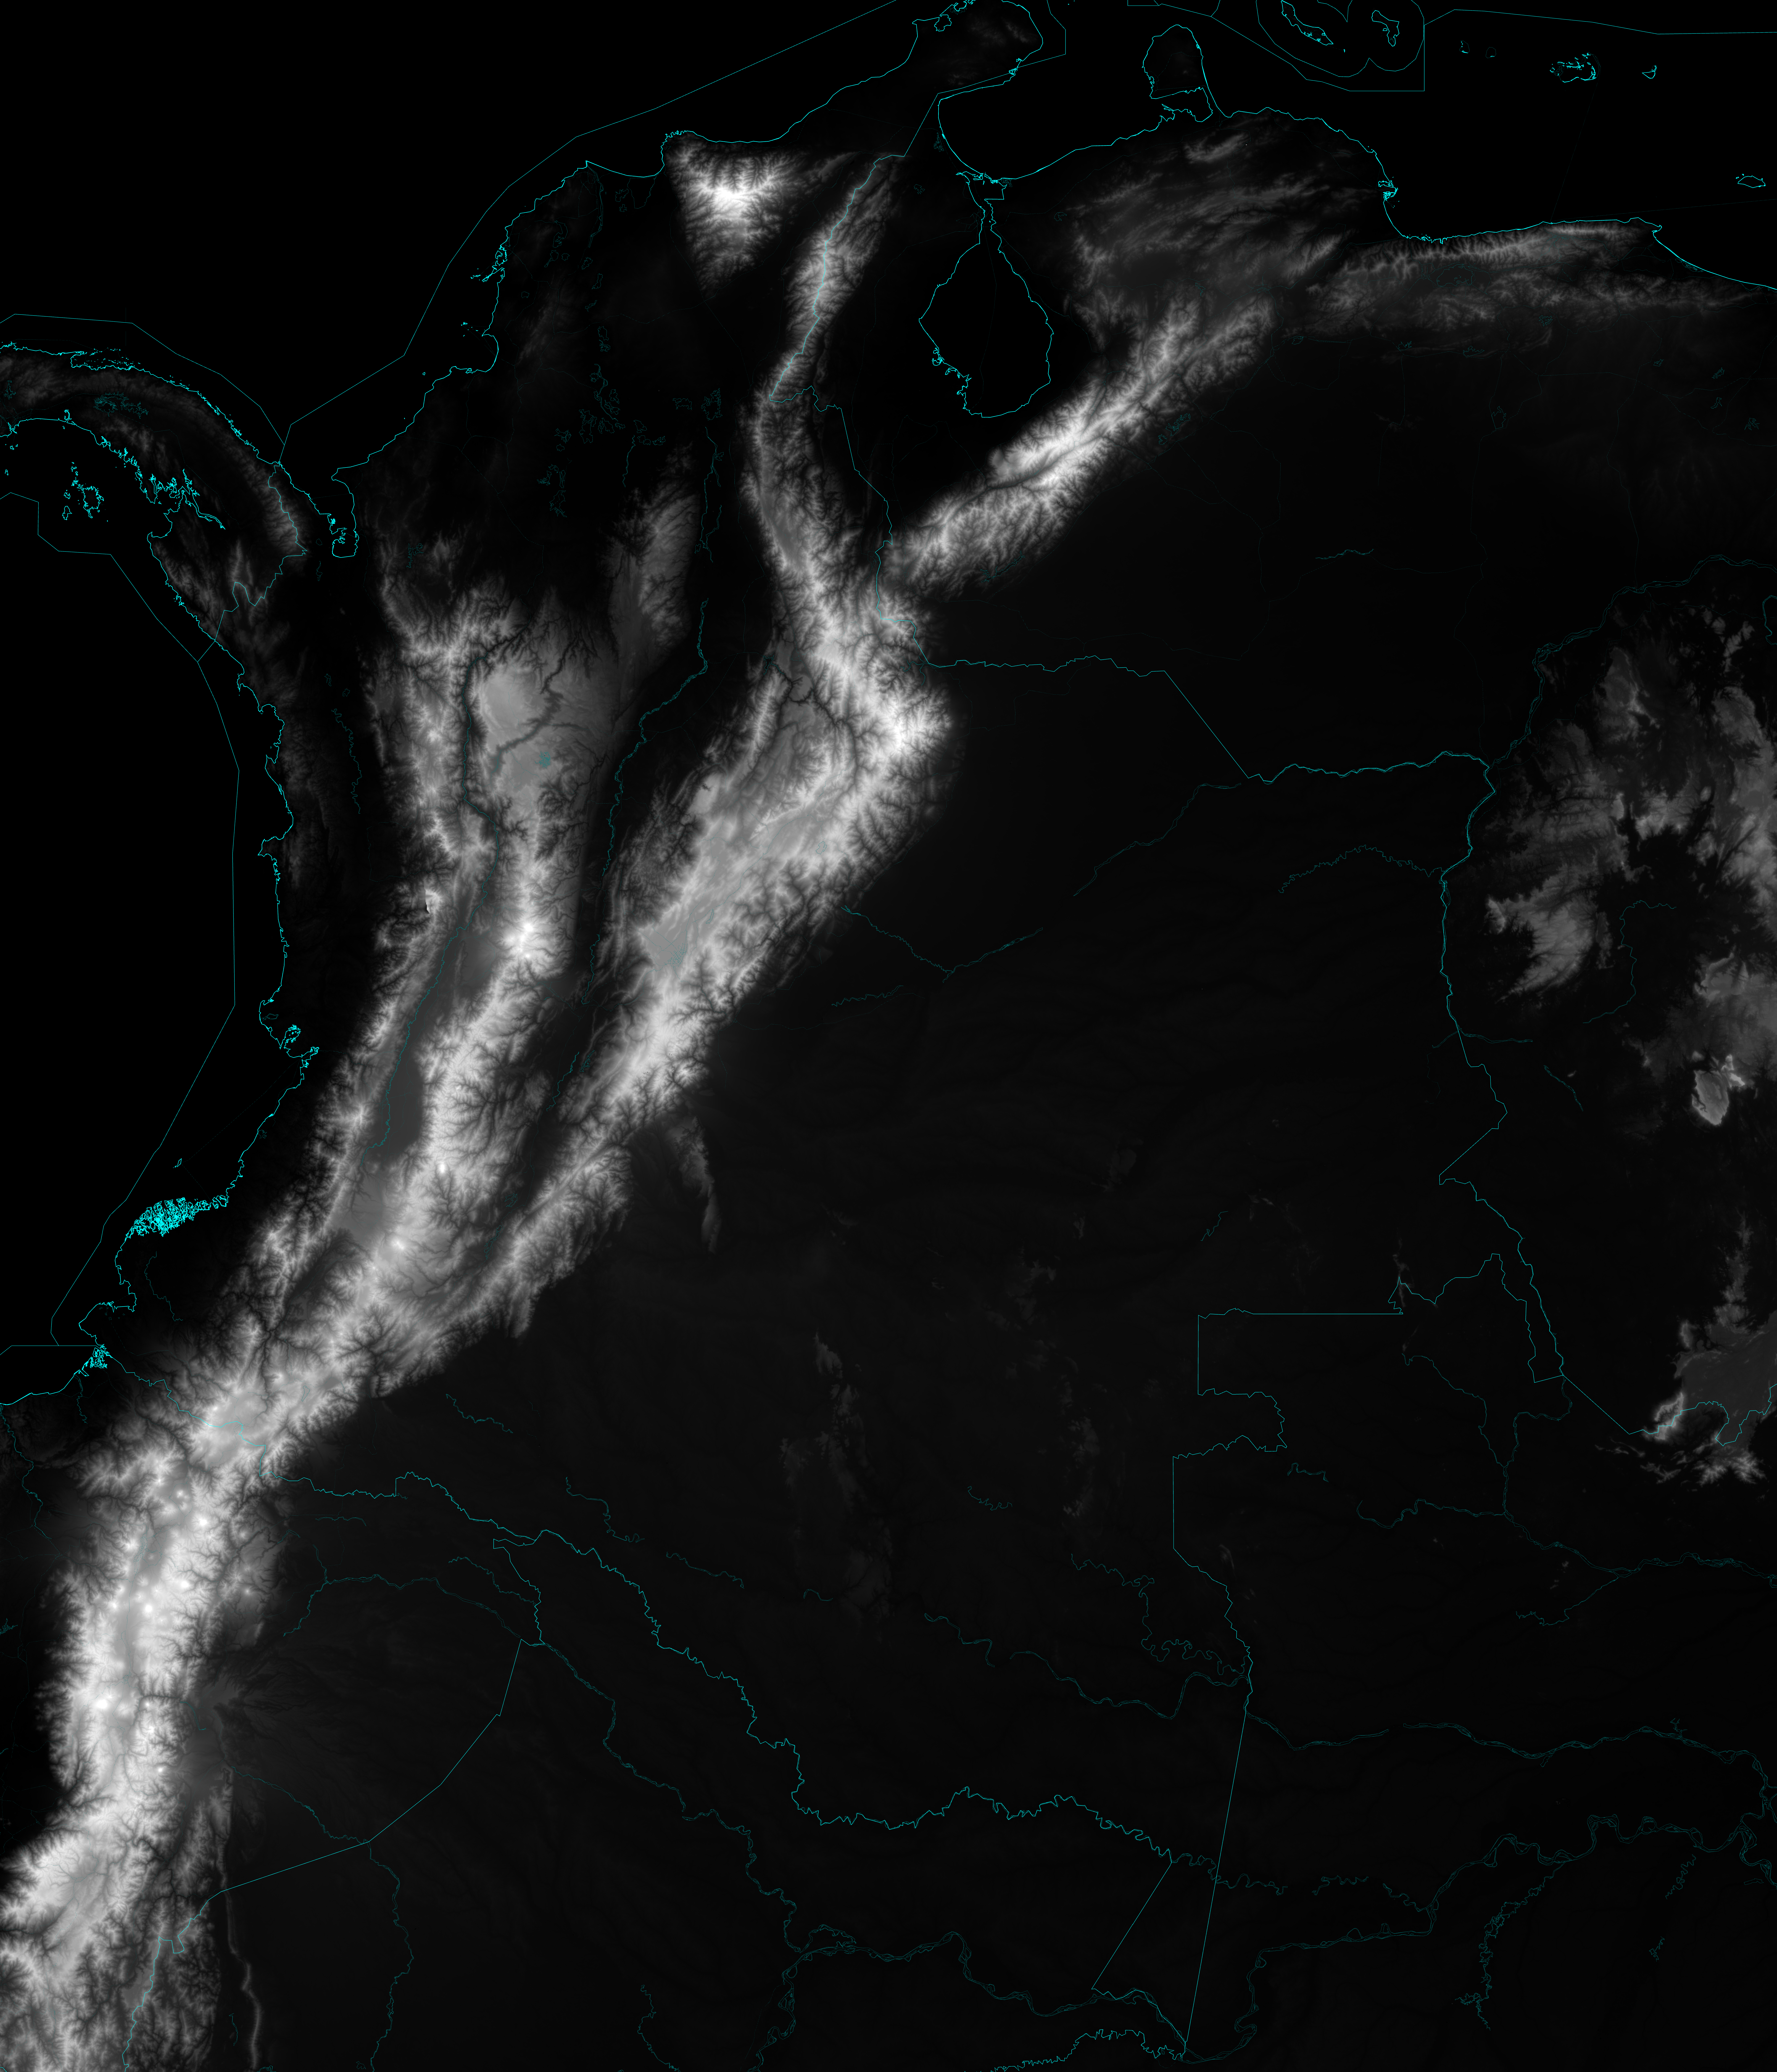
\includegraphics[width=\linewidth]{figures/mapa_alturas.png}
    \caption*{(a) Mapa de elevación en escala de grises.}
\end{minipage}\hfill
\begin{minipage}{0.45\textwidth}
    \centering
    \includegraphics[width=\linewidth]{figures/mapa_colombia_v1.jpeg}
    \caption*{(b) Modelo tridimensional generado en Blender.}
\end{minipage}
\caption{Generación del terreno mediante mapa de elevación en Blender.}
\label{fig:mapa-altura}
\end{figure}

Sin embargo, el modelo obtenido presentaba una alta densidad de polígonos, con un total de 24.5 millones de vértices, como se muestra en la Figura \ref{fig:rendimiento-terreno}.
Debido a ello, durante las pruebas se registró una tasa de cuadros por segundo (\textit{frames per second}, FPS) promedio de 25.9, valor considerablemente inferior al rango óptimo de 30 a 60 FPS recomendado para garantizar una experiencia fluida.
Este rendimiento reducido afectaba tanto el desempeño real del sistema como la percepción del usuario, generando una sensación de lentitud e inestabilidad en la simulación.
\begin{figure}[H]
\centering
\includegraphics[width=0.8\textwidth]{figures/bajo_rendimiento.jpeg}
\caption{Ejemplo del alto número de polígonos del modelo 3D que afecta el rendimiento.}
\label{fig:rendimiento-terreno}
\end{figure}

Esta situación evidenció que el uso de un modelo tridimensional completo para representar el terreno no era una solución óptima, especialmente considerando los requerimientos de eficiencia y fluidez del entorno de simulación.
Por ello, se decidió implementar un método alternativo, que anteriormente desconocíamos, de generación del mapa, con el fin de mejorar la eficiencia y el rendimiento general del entorno virtual.
\subsubsection{Vías}
En un intento por optimizar el proceso de generación del trazado ferroviario, se exploró inicialmente la posibilidad de representar las vías mediante la conexión de puntos y segmentos rectos.
Este enfoque, aunque sencillo en su concepción, requería una gran cantidad de puntos para lograr una precisión adecuada en curvas y pendientes, lo cual incrementaba la complejidad del sistema y afectaba el rendimiento general.
Ante esta limitación, se consideró el uso de \textit{splines}, una técnica matemática que permite la creación de curvas suaves a partir de un conjunto reducido de puntos de control.
Las splines resultan especialmente adecuadas para la representación de vías férreas, ya que facilitan la generación de trayectorias continuas y realistas sin necesidad de definir manualmente cada punto intermedio, mejorando así tanto la precisión geométrica como la eficiencia del proceso de renderizado.
%le añadimos las columnas a los riesgos, con una nueva *tabla de de que tanto riesgo hay* y con eso definimos la columna nivel de riesgo y pues se pone la tabla entera ahora si, lo hemos puesto abierto y cerrado si ya esta hecho
%que este cerrado es que ya se soluciono o se acepto, como los de poco riesgo, que puede..... osea existen cerrados que es porque el problema es muy minimo, no es tan grave

\subsection{Refinación de la lista de riesgos}

Para mejorar la comprensión y categorizar adecuadamente los posibles riesgos presentados en la sección \textit{PONER PRIMERA SECCIÓN DONDE SE 
PRESENTA EL DOC DE RIESGOS}, se diseñó un sistema de evaluación de riesgos compuesto por dos tablas complementarias.
En primer lugar, se definió un rango de niveles de riesgo, donde se definen los valores numéricos del 1 al 5 que representan la magnitud del impacto y la probabilidad de ocurrencia de un evento.
En esta escala, el valor 1 indica una afectación mínima o poco probable, mientras que el valor 5 corresponde a un evento con consecuencias críticas o de alta probabilidad, tal como se explica en la Figura \ref{fig:linea_impacto_probabilidad}.
\begin{figure}[H]\centering
  \includegraphics[width=\linewidth]{figures/linea de impacto-probabilidad.png}
  \caption{Rango de riesgos y Probabilidad.
Fuente: Propia}
  \label{fig:linea_impacto_probabilidad}
\end{figure}

En segundo lugar, se desarrolló una tabla general de riesgos, en la que se registran los posibles problemas identificados durante el proyecto.
Esta tabla incluye los campos Descripción (donde se detalla el problema detectado), Causa, Impacto, Probabilidad, Nivel de riesgo (calculado como el producto del impacto con la probabilidad), Plan de acción (estrategias o medidas a tomar) y Estado (donde se especifica si el riesgo permanece abierto o ya ha sido cerrado).
En la tabla \ref{tab:matriz-riesgos} se muestra el artefacto entregado.

Hay que aclarar que, algunos riesgos se mantuvieron abiertos incluso hasta el final del desarrollo del proyecto.
Esto se debe a que se consideró que el nivel de riesgo era suficientemente bajo como para evitar gastar recursos en solucionarlo.
\begin{landscape}
\begin{longtable}{|c|L{2.8cm}|L{2.8cm}|c|c|c|L{3.2cm}|c|}
\caption{Matriz de riesgos del proyecto}\label{tab:matriz-riesgos} \\
\hline
\multicolumn{1}{|c|}{\textbf{No. Ref}} &
\multicolumn{1}{c|}{\textbf{Descripción}} &
\multicolumn{1}{c|}{\textbf{Causa}} &
\multicolumn{1}{c|}{\textbf{Impacto}} &
\multicolumn{1}{c|}{\textbf{Probabilidad}} &
\multicolumn{1}{c|}{\textbf{Nivel de Riesgo}} &
\multicolumn{1}{c|}{\textbf{Plan de acción}} &
\multicolumn{1}{c|}{\textbf{Estado}} \\
\hline
\endfirsthead

\hline
\multicolumn{1}{|c|}{\textbf{No.
Ref}} &
\multicolumn{1}{c|}{\textbf{Descripción}} &
\multicolumn{1}{c|}{\textbf{Causa}} &
\multicolumn{1}{c|}{\textbf{Impacto}} &
\multicolumn{1}{c|}{\textbf{Probabilidad}} &
\multicolumn{1}{c|}{\textbf{Nivel de Riesgo}} &
\multicolumn{1}{c|}{\textbf{Plan de acción}} &
\multicolumn{1}{c|}{\textbf{Estado}} \\
\hline
\endhead

R1 & El modelo del terreno del mapa de Colombia está mal optimizado & El uso de modelo 3D genera una sobrecarga en la memoria gráfica & 4 & 4 & 16 & Realización de un terreno formal de Unity sin usar Blender.
Carga de terreno por bloques. & Cerrado \\ \hline
R2 & La cámara del jugador puede atravesar el terreno.
& La cámara no está programada para evadir o chocar con el mapa.
& 2 & 5 & 10 & Implementación de una función para aplicar una colisión de cámara con el terreno y evitar el paso.
& Abierto \\ \hline
R3 & Las vías se generan de manera poco natural e inconexa.
& Uso de puntos y rectas para la asignación de vías & 5 & 4 & 20 & Cambiar a uso de spline.
& Cerrado \\ \hline
R4 & Terreno con parches o incoherencias.
& El DEM utilizado está con ciertos datos erróneos o vacíos.
& 2 & 3 & 6 & Cambiar de DEM o arreglar los parches haciendo uso de algoritmos.
& Cerrado \\ \hline
R5 & Textura de vías solapando suelo en plano.
& Vía colocada en el punto exacto donde está el terreno, generando solapamiento & 1 & 2 & 2 & Mover las vías generadas una pequeña distancia hacia arriba & Cerrado \\ \hline
R6 & Las vías no permiten al tren dar vueltas en un circuito cerrado.
& Spline no cerrado & 2 & 3 & 6 & Añadir que el circuito detecte cuando se colocan vías cerca al punto inicial, y de ser así cierre el circuito & Cerrado \\ \hline
R7 & Dificultad para representar todos los ríos y lagos de Colombia en el mapa.
& Colombia tiene una gran densidad de elementos hidrológicos, que superan la capacidad de representación fiel en el terreno del videojuego.
& 4 & 4 & 16 & Definir criterios de selección: incluir solo ríos principales y lagos mayores.
& Abierto \\ \hline
R8 & Las vías atraviesan montañas & La generación de vías no interpola dichas alturas & 3 & 4 & 12 & Modificar la función de generación de vías, para que, cuando la vía atraviese el terreno, genere un túnel en la zona atravesada.
& Cerrado \\ \hline
R9 & Estadísticas de las locomotoras no son leídas correctamente & Estadísticas guardadas en los GameObject hijos de la Locomotora & 4 & 2 & 8 & Unificar la lógica y estadísticas de las distintas locomotoras en el GameObject padre Locomotora & Cerrado \\ \hline
R10 & HUD no muestra la vida actual del tren al hacer cambio de locomotora & Dato de vida y estadísticas no leído después del cambio & 2 & 2 & 4 & Crear una función para reiniciar las estadísticas del tren & Cerrado \\ \hline
R11 & Modelos 3D de los trenes y 
ciudades se ven a escalas diferentes & Escalas y rotaciones no aplicadas correctamente en Blender & 1 & 3 & 3 & Aplicar escalas y rotaciones a los modelos 3D de los trenes y ciudades & Cerrado \\ \hline
R12 & Shaders incompatibles y LOD's mal configurados.
& Unity tiene valores por defecto en las generaciones de terreno que no siempre es compatible entre shaders y capas de niveles de detalle.
& 3 & 3 & 9 & Testear y ajustar shaders, URP, en diferentes escenarios, hasta llegar a la configuración correcta.
& Cerrado \\ \hline
R13 & El videojuego puede andar en muy bajos FPS en los equipos de cómputo de los usuarios.
& Al desarrollar el proyecto en equipos con especificaciones mayores a la media, se omite algunos aspectos de optimización.
& 5 & 3 & 15 & Investigar las especificaciones de los equipos donde se realizará la prueba y reevaluar riesgos.
& Abierto \\ \hline
\end{longtable}
\end{landscape}

%al final si van las HU completas, 
%añadir una fase extra para colocar el diagrama de actividades inicial (el diagrama de actividades es mental)y el diagrama de componentes *el UML grande q urbano ni miró*, hay que explicarlo por partes por lo gigante

Finalmente, se asignaron a las historias de usuario la técnica de priorización MoSCoW, enfocando el proyecto en lo más valioso y viable.
Clasifica en: Must have (imprescindible), Should have (importante), Could have (deseable si hay recursos) y Won’t have (no se hará por ahora).
Así mismo, se estableció la variable de cumplimiento, con valores comprendidos entre 0 y 1, donde 0 indica que la actividad no se ha iniciado y 1 que ha sido completada en su totalidad, este no fue agregado en la Tabla \ref{tab:HU-epica} ya que todos fueron cumplidos.
Por último, se definió el nivel de complejidad, con una escala de 1 a 5, en la cual 1 corresponde a tareas de baja dificultad y 5 a aquellas de mayor complejidad.
\begin{landscape}
\begin{longtable}{|M{1.2cm}|M{1.8cm}|L{8cm}|M{2.2cm}|M{2cm}|}
\caption{Tabla final de historias de usuario.} \label{tab:HU-epica} \\
\hline
\multicolumn{1}{|c|}{\textbf{ÉPICA}} &
\multicolumn{1}{c|}{\textbf{CÓDIGO}} &
\multicolumn{1}{c|}{\textbf{HISTORIA DE USUARIO}} &
\multicolumn{1}{c|}{\textbf{PRIORIZACIÓN}} &
\multicolumn{1}{c|}{\textbf{COMPLEJIDAD}} \\ \hline
\endfirsthead

\hline
\multicolumn{1}{|c|}{\textbf{ÉPICA}} &
\multicolumn{1}{c|}{\textbf{CÓDIGO}} &
\multicolumn{1}{c|}{\textbf{HISTORIA DE USUARIO}} &
\multicolumn{1}{c|}{\textbf{PRIORIZACIÓN}} &
\multicolumn{1}{c|}{\textbf{COMPLEJIDAD}} \\ \hline
\endhead

\hline
\multicolumn{5}{r}{\textit{Continúa en la siguiente página}} \\
\endfoot

\hline
\endlastfoot

1 & HU1  & Como jugador, quiero ver una pantalla de selección de niveles para elegir cuál jugar.
& M & 2 \\ \hline
1 & HU2  & Como jugador, quiero que al empezar un nivel, se me presente una pantalla de contrato que detalle el presupuesto, los objetivos y los posibles desafíos.
& M & 1 \\ \hline
2 & HU3  & Como jugador, quiero poder mover la cámara (panorámica) por el mapa para explorar el terreno.
& M & 1 \\ \hline
2 & HU4  & Como jugador, quiero poder acercar y alejar la vista (zoom) para ver el mapa con diferentes niveles de detalle.
& M & 1 \\ \hline
2 & HU5  & Como jugador, quiero ver las delimitaciones políticas y ríos.
& M & 3 \\ \hline
2 & HU6  & Como jugador, quiero ver un terreno del nivel a jugar.
& M & 4 \\ \hline
2 & HU7  & Como jugador, quiero poder rotar la cámara para observar el terreno desde distintos ángulos.
& S & 1 \\ \hline
2 & HU8  & Como jugador, quiero poder activar una capa de vista topográfica para entender el relieve del terreno.
& C & 5 \\ \hline
3 & H10  & Como jugador, quiero poder construir un tramo de vía férrea entre dos puntos.
& M & 2 \\ \hline
3 & H11  & Como jugador, quiero poder eliminar un tramo de vía férrea para rediseñar mis rutas.
& M & 1 \\ \hline
3 & HU12 & Como jugador, quiero que se pueda construya un puente o valles.
& M & 4 \\ \hline
3 & HU13 & Como jugador, quiero que se construya automáticamente un túnel si mi vía férrea atraviesa una montaña.
& M & 4 \\ \hline
3 & HU14 & Como jugador, quiero poder construir estaciones en puntos específicos de la vía para definir los puntos de inicio y fin del ciclo.
& M & 3 \\ \hline
3 & HU15 & Como jugador, quiero que la interfaz muestre mi presupuesto actual en todo momento para controlar mis gastos de construcción.
& M & 2 \\ \hline
3 & HU16 & Como jugador, quiero poder deshacer mi última acción de construcción para corregir un error rápidamente.
& S & 2 \\ \hline
4 & HU17 & Como jugador, tras diseñar la ruta, quiero acceder a un menú para seleccionar y comprar la locomotora que usaré.
& M & 3 \\ \hline
4 & HU18 & Como jugador, quiero poder añadir vagones específicos (pasajeros, carga) a mi locomotora para cumplir los requisitos del contrato.
& M & 2 \\ \hline
4 & HU19 & Como jugador, quiero que el menú de selección me muestre las locomotoras de la ruta que diseñé.
& C & 2 \\ \hline
5 & HU20 & Como jugador, durante la simulación, quiero ver una alerta o efecto visual cuando un tren está sufriendo daños al pasar por una zona de evento.
& M & 2 \\ \hline
5 & HU21 & Como jugador, quiero que el botón de "Hacer Testeo" me informe si me falta algún requisito para iniciar la simulación.
& S & 3 \\ \hline
5 & HU22 & Como jugador, quiero tener la opción de volver a la fase de construcción después de un testeo para modificar mis rutas antes de la evaluación final.
& S & 1 \\ \hline
6 & HU23 & Como jugador, al finalizar un nivel, quiero ver una pantalla de puntuación que califique mi desempeño.
& M & 3 \\ \hline
6 & HU24 & Como jugador, quiero que mi puntuación final considere la rentabilidad (costo total vs. valor del contrato).
& M & 3 \\ \hline
6 & HU25 & Como jugador, quiero que mi puntuación final considere la durabilidad (estado final de mis trenes y vías tras la simulación).
& M & 3 \\ \hline
6 & HU26 & Como jugador, quiero que mi puntuación final considere la eficiencia (tiempo que tardó el tren en completar el ciclo).
& S & 3 \\ \hline
6 & HU27 & Como jugador, quiero ver un informe detallado que desglose mi puntuación final para entender cómo mejorar.
& S & 3 \\ \hline
7 & HU28 & Como jugador, quiero que se desbloqueen nuevos niveles en el menú de selección tras completar el contrato actual.
& M & 2 \\ \hline
8 & HU29 & Como jugador, quiero que Don Raíl me presente el contrato al inicio de cada nivel con un diálogo breve, para darme un objetivo narrativo y contexto histórico sobre la región.
& S & 3 \\ \hline
8 & HU30 & Como nuevo jugador, quiero que Don Raíl me guíe a través de un tutorial interactivo en el primer nivel, para aprender las mecánicas del juego de una forma amigable y contextual.
& S & 4 \\ \hline
8 & HU31 & Como jugador, quiero que Don Raíl me dé una advertencia contextual si construyo una vía con una pendiente muy pronunciada o una curva muy cerrada, para que pueda corregir errores de ingeniería antes del testeo.
& S & 4 \\ \hline
8 & HU32 & Como jugador, quiero que al seleccionar una estación o ciudad importante, aparezca un ícono de Don Raíl que pueda clickear para escuchar un dato histórico sobre la importancia ferroviaria de ese lugar.
& S & 4 \\ \hline
8 & HU33 & Como jugador, quiero escuchar o leer un breve comentario de Don Raíl cuando un tren sufre un evento durante la simulación, para aumentar la inmersión.
& S & 3 \\ \hline
8 & HU34 & Como jugador, quiero que Don Raíl comente sobre mi puntuación final, celebrando el éxito con emoción o dándome un consejo en caso de fallar para que la evaluación se sienta más personal.
& S & 2 \\ \hline
8 & HU35 & Como jugador, quiero que durante las pantallas de carga, aparezcan anécdotas cortas o "dichos" de Don Raíl sobre la vida en el ferrocarril, para enriquecer el mundo del juego y aprovechar los tiempos de espera.
& M & 2 \\ \hline
6 & HU36 & Como administrador, quiero adquirir y guardar metadatos de los jugadores en una base de datos para poder generar informes.
& M & 3 \\ \hline

\end{longtable}
\end{landscape}



\section{Implementación}
% (Completar) vendria a ser implementacion
poner el tablero kanban, hay que inventarse que hizo cada uno pq no hay registro, tiene que tener semanas, inventadas si no recordamos / tipo semana 1, semana 2, semana 3-5, semana 6 a 7 y asi hasta que la columna de finalizado este completa.
mejor dicho de la semana tal a tal se hizo esto, de esta a esta se hizo esto.
poner entre semanas y narrar un poco el progreso, sucedieron estos problemas, decidimos hacer ciertos cambiso a tal cosa

hay mas libertad la vdd, asi q esto es un comodin *BALATRO REFERENCIA*

estaria bien colocar el diagrama de componentes aca si terminado final y explicado a detalle

\section{Pruebas}
% (Completar) vendria a ser evaluacion

publicarlo en internet

obtener resultados de envuesta de jugadores

analizar los resultados, nadie jugo el 3 nivel, pirobos

*unificar actividades* A1 

% Bibliografía
\printbibliography[title={Referencias}]

% (Opcional) Apéndices
% \appendix
% \include{appendices/apendice-a}

\end{document}
